%!TEX root = ../../thesis.tex

\subsubsection{Reduction issues}
\label{subsubsec:reductionartefacts}
\textbf{\todo{After X thing}{At a later date}} some large artefacts in the {DRACS} extracted spectra were identified.
An investigation into the cause of these artefacts was undertaken to identify their source and remove them from the spectra.
Separating out the individual nod spectra side-by-side revealed that the artefacts were occurring in only a few of the individual nod spectra from the optimal extraction, and that they were not present in the rectangular extracted nods. \textbf{Four} examples are shown in \textbf{\cref{fig:resizednods} and blah}.
In each panel the top sub-plot contains the optimal extracted spectra, while the middle sub-plot contains the rectangularly extracted spectra.


The occurrence of artefacts in the observations did not appear to have a pattern with nod position or detector. \textbf{They do occur with large spikes in the rectangular extractions.
There are many other spikes in the rectangular extractions that do not create the artefacts observed.
}\todo{this doesn't quite flow}
It is clear that the artefacts in the optimally extracted nods correspond to large pixel spikes present in the rectangular extracted nod.
As mentioned in \cref{subsec:extraction} the \emph{optimal} extraction includes variance weighting across the spatial direction.
It appears that the presence of cosmic rays or bad pixels heavily affected the variance weighting procedure during the \emph{optimal} extraction.
It is also observed that the artefacts created are not localized to the region around the bad pixel region but affect an extended spectral range (100's of pixels in some cases).

Numerous parameters in the {DRACS} pipeline were experimented with to try and remove the observed artefacts with limited success.
For instance, no complete removal of the artefacts was found by manually changing the \(\sigma\) rejection limits (between \(1-5 \sigma\)) and increasing the tracing width parameter in {IRAF}s DOSLIT\footnote{Documentation for DOSLIT can be found here \href{http://stsdas.stsci.edu/cgi-bin/gethelp.cgi?doslit}{http://stsdas.stsci.edu/cgi-bin/gethelp.cgi?doslit}} recipe, although it did slightly affect the shape of the artefacts.
During the creation of this document it was discovered that enabling the automated aperture resizing\footnote{Using \href{apresize}{http://stsdas.stsci.edu/cgi-bin/gethelp.cgi?apresize.hlp}} by setting the ``resize'' parameter to yes manages to remove one of the large artefacts in the observation of {HD202206-1}.
The effect of this is shown in \cref{fig:resizednods} with the optimal and rectangular extraction from the {DRACS} pipeline with only the ``resize'' parameter changed.
The artefact in the \nth{6} nod is removed by enabling the automatic ``resize'' but the artefact in the \nth{7} nod is still present.

\begin{figure}
    \centering
    \begin{tabular}{cc}
        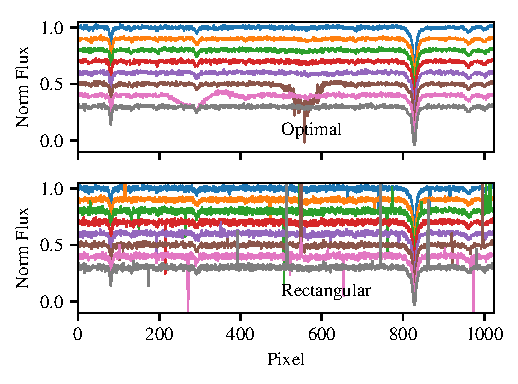
\includegraphics[width=0.5\linewidth]{figures/reduction/bp_plots/non_resized_nods_HD202206-1_chip_2} & 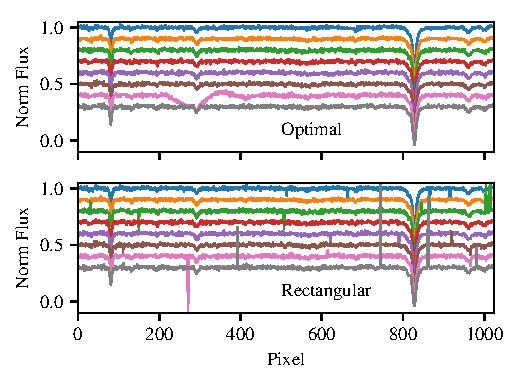
\includegraphics[width=0.5\linewidth]{figures/reduction/bp_plots/resized_nods_HD202206-1_chip_2}\\
    \end{tabular}
    \caption{{DRACS} reduction for detector \#2 of HD202206-1 with a single pipeline parameter changed.
        Left: Reduction with the DRACS pipeline with the ``doslit.resize'' set to ``no''.
        Right: The reduction from the same pipeline but with ``doslit.resize'' set to ``yes''.
        During the order tracing the aperture size is automatically adjusted while the rest of the parameters remain identical.
        With this one parameter changed one large artefact is removed but a second one is not removed.}
    \label{fig:resizednods}
\end{figure}

This discovery came too late to implement for all of the observations as it would require all of the analysis to be repeated re-doing all of the analysis.
However, it does indicate that some improvements may be obtained with extensive time and patience tweaking the parameters of the {DRACS} pipeline.

The artefacts in the individual nod spectra were observed to create flux deviations in the fully combined optimally extracted spectra of around \(0.5\%\).
The purpose of these spectra was to detect faint companion spectra with expected flux ratios \(\rm {F_2}/{F_1} < 1\%\).
Therefore, measures are needed to remove these artefacts from the combined spectra.

The solution that was chosen was to replace the optimally extracted nods that contained artefacts with their rectangular counterparts, creating a combined spectra that had a mix of optimally reduced and rectangularly reduced nod spectra.
To replace the spikes in the rectangular extraction that created the artefacts and others an iterative 4-\(\sigma\)\footnote{There is no scientific justification why 4-\(\sigma\) was chosen over the commonly used 3-\(\sigma\).} rejection algorithm\footnote{Found at \url{https://github.com/jason-neal/nod_combination}} was applied to the rectangular extractions.
The \(\sigma\) for each pixel was calculated as the standard deviation of the nearest 2 pixels on either side of it, across all 8 nod spectra.
Any rejected pixels were replaced using linear interpolation along the spectra.


Combined spectra were finally constructed by averaging the eight nod-cycle spectra together, where some of the optimally extracted spectra were replaced using the above method. \textbf{The third panel of \cref{fig:badpixelreplacement} shows the difference between the combined spectra using only optimally extracted spectra and the mixed combination with replacements.} The actual spectra from the two different methods can be seen in \cref{fig:reduction-comparison} where orange is the combination of optimally reduced spectra only and green uses the replacement method outlined here.


\todo{This needs to be fixed up with a different plot, possibly even removed as there are examples in appendix}
\textbf{There is a clear large extended artefact on the \nth{7} nod of the top panel is created by the large spike.
    For the first panel a single large spike in the \nth{7} nod (pink) near pixel 230 creates a wide and noticeable artefact in the optimal extraction.
    This is the same spectra as the \nth{2} down the right of \cref{fig:reduction-comparison}.
}

\textbf{
    EXAMPLE with the new-old \cref{fig:badpixelreplacement}}.
\todo{CHANGE the figure here}
\begin{figure}
    \centering
    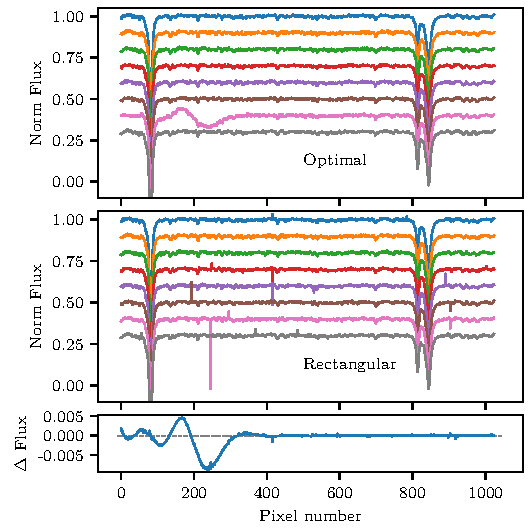
\includegraphics[width=\hsize/2]{figures/reduction/bp_plots/Bad_pixel_replacement}
    \caption{Example of an artefact in the optimally extracted spectra from detector \#2 of {\red{} HDXXXXXX}.
        The top panel contains the 8 normalized nod spectra obtained using optimal extraction.
        The middle panel shows the same nod spectra reduced using only rectangular extraction.
        The bottom panel shows the difference between a combined spectrum using optimal nods only and a combined spectrum in which the identified nods are replaced with their rectangular counterparts as per \cref{subsubsec:reductionartefacts}.
        A vertical offset is included between each spectra for clarity.
        The nod spectra are in observation order from top to bottom.}
    \label{fig:badpixelreplacement}
\end{figure}

The percentage of individual nod spectra from all detectors and observations affected by artefacts was 14\%.
These are detailed in \cref{tab:nod_replacement}.
More examples of observations that contain artefacts are given in \cref{appendix:artefacts}, selected to show a variation in appearance.


The continuum normalization is performed in {IRAF} while the mixed combination is carried out in \emph{Python} along with the post reduction procedures detailed below.
This pipeline was chosen over the {ESO} {CRIRES} pipeline because it seemed relatively simpler to use, being semi-automated, and appeared to have less bad pixel/cosmic ray artefacts in the resulting spectra.
In hindsight the artefacts that appeared in the {DRACS} reduction took longer to investigate and create a solution for.
The solution involved a script to remove the bad pixels that created the artefacts.
The avoidance of bad pixels and the creation of a removal code, was one of the original choices for using the {DRACS} pipeline instead of the {ESO} pipeline.


One hypothesis for these artefacts is detector glow, a heating of the detector by the nearby amplifiers in the chip (see \cref{subsubsec:darkcurrent}\todo{check correct section}).
\unfinished{check this statement}{The artefacts in the \emph{K}-band spectra were not observed in previous works in the \emph{H}-band using this pipeline~\citep[e.g.][]{figueira_radial_2010}, and as such may have a wavelength dependent effect, like detector glow.
    However, this no longer seems plausible as the location of the artefacts do not seem to indicate a pattern corresponding to the shape of the glow shown in \cref{fig:darkcurrent_colour}.
    It could also be that there were artefacts in intermediate steps of the previous works that were missed due to the semi-automated pipeline, with the resultant combined spectrum being only slightly affected.}
Anther possibility is that the artefacts are bad pixels not removed correctly.
Regardless, they do not have a significant impact on the results found in this work, though it is expected that that mixing optimally reduced spectra with rectangularly reduced spectra will have a slight negative impact on the noise or \snr{} of the combined spectrum.


Much time and effort went into trying to extract the spectra as best as possible, without artefacts, to have the best chance at obtaining high quality scientific results of the faint features sought after in this work.
Due to time constraints the replacement of nods with artefacts (indicated in \cref{tab:nod_replacement}) with their rectangular counterparts was performed.
